% Generated by paper/build_imt_parameter_figures.py; do not hand edit.
% Q1 grid SHA-256: 1a48a6f4d5a4c6c1449f35cd7e5584b7a14d4a08f8effc2c4508497e8ef20058
\begin{figure}[tb]
\centering
\begin{minipage}[t]{.485\linewidth}
\centering
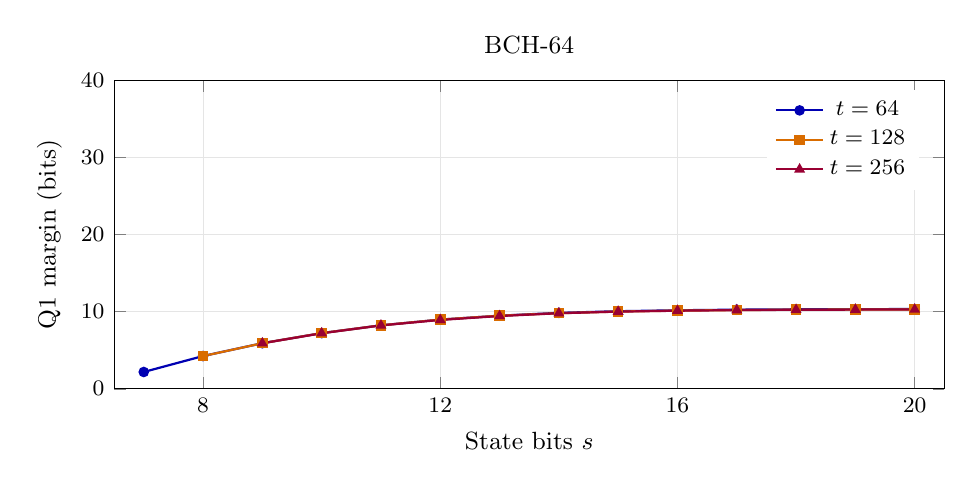
\begin{tikzpicture}
\begin{axis}[tick label style={font=\footnotesize},label style={font=\small},title style={font=\small},grid=major,grid style={black!10},legend style={font=\footnotesize,draw=none},width=\linewidth,height=5.5cm,title={BCH-64},xlabel={State bits $s$},ylabel={Q1 margin (bits)},xmin=6.5,xmax=20.5,ymin=0,ymax=40,xtick={8,12,16,20},legend pos=north east,]
\addplot[blue!70!black,thick,mark=*,mark size=1.5pt] coordinates {(7,2.1827116585) (8,4.2514093897) (9,5.9147821095) (10,7.2247246256) (11,8.2306365668) (12,8.9772543375) (13,9.4838898435) (14,9.8505560891) (15,10.0610100645) (16,10.1847253778) (17,10.2642828362) (18,10.3073487861) (19,10.3292263422) (20,10.3403771086)};
\addlegendentry{$t=64$}
\addplot[orange!85!black,thick,mark=square*,mark size=1.5pt] coordinates {(8,4.2430472521) (9,5.9129395061) (10,7.2224925389) (11,8.2281561682) (12,8.9741001763) (13,9.4805569735) (14,9.8077200834) (15,10.0175657415) (16,10.1370857462) (17,10.2158805444) (18,10.2589462533) (19,10.2808187416) (20,10.2919600489)};
\addlegendentry{$t=128$}
\addplot[purple!80!black,thick,mark=triangle*,mark size=1.5pt] coordinates {(9,5.9089535105) (10,7.2018221055) (11,8.2229102705) (12,8.9322403044) (13,9.4387211691) (14,9.7997939364) (15,10.0090784426) (16,10.1270377235) (17,10.2050661704) (18,10.2479773575) (19,10.2698512751) (20,10.2808321532)};
\addlegendentry{$t=256$}
\end{axis}
\end{tikzpicture}
\end{minipage}
\hfill
\begin{minipage}[t]{.485\linewidth}
\centering
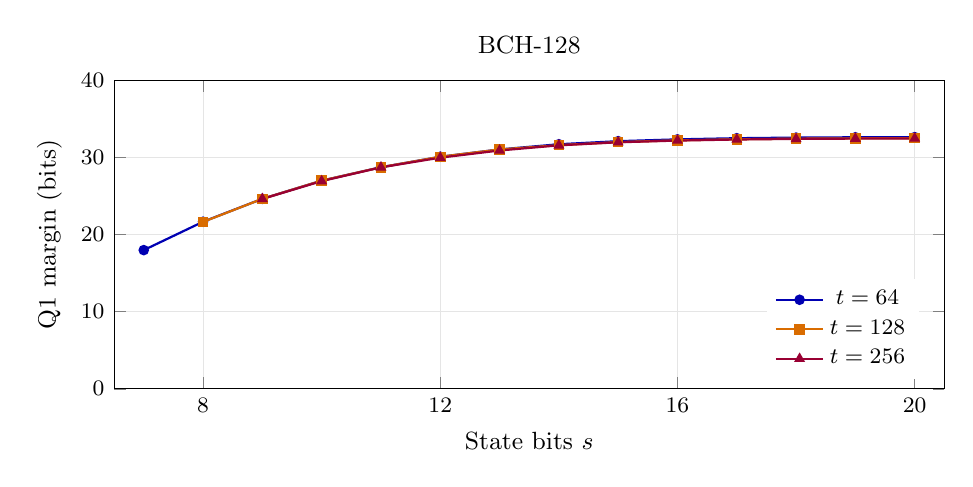
\begin{tikzpicture}
\begin{axis}[tick label style={font=\footnotesize},label style={font=\small},title style={font=\small},grid=major,grid style={black!10},legend style={font=\footnotesize,draw=none},width=\linewidth,height=5.5cm,title={BCH-128},xlabel={State bits $s$},ylabel={Q1 margin (bits)},xmin=6.5,xmax=20.5,ymin=0,ymax=40,xtick={8,12,16,20},legend pos=south east,]
\addplot[blue!70!black,thick,mark=*,mark size=1.5pt] coordinates {(7,17.9834453302) (8,21.6621321145) (9,24.6347504734) (10,26.9894832727) (11,28.7304904965) (12,30.0911153162) (13,31.0377180335) (14,31.7087951291) (15,32.1068469089) (16,32.3411624023) (17,32.4919665503) (18,32.5706569452) (19,32.6109835173) (20,32.6317852093)};
\addlegendentry{$t=64$}
\addplot[orange!85!black,thick,mark=square*,mark size=1.5pt] coordinates {(8,21.6399383579) (9,24.6317302099) (10,26.9854051669) (11,28.7251108759) (12,30.0842904573) (13,31.0283485223) (14,31.5876633568) (15,31.9847921817) (16,32.2093340249) (17,32.3546170480) (18,32.4330203557) (19,32.4731496421) (20,32.4935511435)};
\addlegendentry{$t=128$}
\addplot[purple!80!black,thick,mark=triangle*,mark size=1.5pt] coordinates {(9,24.6251404652) (10,26.9311396417) (11,28.7137024495) (12,29.9699710581) (13,30.9001510687) (14,31.5677999653) (15,31.9634354456) (16,32.1865537842) (17,32.3248385177) (18,32.4027324343) (19,32.4425635106) (20,32.4626971764)};
\addlegendentry{$t=256$}
\end{axis}
\end{tikzpicture}
\end{minipage}
\caption{IMT state and step size at $K=2^{20}$. Each $t$ uses its own nested
map chain. More state gives diminishing Q1 gains; the step-size curves
nearly coincide at shared states.}
\label{fig:finite-s-t}
\end{figure}
